% !TEX TS-program = pdflatex
% !TEX encoding = UTF-8 Unicode

% This is a simple template for a LaTeX document using the "article" class.
% See "book", "report", "letter" for other types of document.

\documentclass[11pt]{article} % use larger type; default would be 10pt

\usepackage[utf8]{inputenc} % set input encoding (not needed with XeLaTeX)

%%% Examples of Article customizations
% These packages are optional, depending whether you want the features they provide.
% See the LaTeX Companion or other references for full information.

%%% PAGE DIMENSIONS
\usepackage{geometry} % to change the page dimensions
\geometry{a4paper} % or letterpaper (US) or a5paper or....
% \geometry{margin=2in} % for example, change the margins to 2 inches all round
% \geometry{landscape} % set up the page for landscape
%   read geometry.pdf for detailed page layout information

\usepackage{graphicx} % support the \includegraphics command and options

% \usepackage[parfill]{parskip} % Activate to begin paragraphs with an empty line rather than an indent

%%% PACKAGES
\usepackage{booktabs} % for much better looking tables
\usepackage{array} % for better arrays (eg matrices) in maths
%\usepackage{paralist} % very flexible & customisable lists (eg. enumerate/itemize, etc.)
\usepackage{verbatim} % adds environment for commenting out blocks of text & for better verbatim
\usepackage{subfig} % make it possible to include more than one captioned figure/table in a single float
% These packages are all incorporated in the memoir class to one degree or another...

%%% HEADERS & FOOTERS
\usepackage{fancyhdr} % This should be set AFTER setting up the page geometry
\pagestyle{fancy} % options: empty , plain , fancy
\renewcommand{\headrulewidth}{0pt} % customise the layout...
\lhead{}\chead{}\rhead{}
\lfoot{}\cfoot{\thepage}\rfoot{}

%%% SECTION TITLE APPEARANCE
\usepackage{sectsty}
\allsectionsfont{\sffamily\mdseries\upshape} % (See the fntguide.pdf for font help)
% (This matches ConTeXt defaults)

%%% ToC (table of contents) APPEARANCE
\usepackage[nottoc,notlof,notlot]{tocbibind} % Put the bibliography in the ToC
\usepackage[titles,subfigure]{tocloft} % Alter the style of the Table of Contents
\renewcommand{\cftsecfont}{\rmfamily\mdseries\upshape}
\renewcommand{\cftsecpagefont}{\rmfamily\mdseries\upshape} % No bold!

%%% END Article customizations

\usepackage[spanish]{babel}
\usepackage{listings} 
%%% The "real" document content comes below...

\title{JS}
%\date{} % Activate to display a given date or no date (if empty),
         % otherwise the current date is printed 

\begin{document}
\maketitle
%\tableofcontents % No hace falta un TOC en un artículo corto


DEBER
INVESTIGACIÓN
\newline
\newline
DE 
\newline
\newline
 LENGUAJES DE PROGRAMACIÓN
\newline
\newline
TEMA:  JAVASCRIPT
\newline
\newline
INTEGRANTES: 
\newline
\newline
DENNISE PINTADO
\newline
\newline
JONATHAN MENDIETA
\newline
\newline
JANINA COSTA
\newline
\newline

\newpage
\title{JS}

\section{Introducción}
La presente investigación es sobre el lenguaje de programación JavaSript  (lenguaje interpretado  dialecto del estándar ECMAScript) definido como un lenguaje orientado a objetos.\\
\\La característica principal de JavaSript es su simplicidad y manejabilidad.\\
\\Para conocer más sobre este lenguaje de programación veremos las características más importantes,  como surgió, los requisitos para su correcta instalación y la forma más sencilla de aprender JavaScript. \\
\\La investigación se realiza por el interés de aprender sobre un nuevo lenguaje el cual nos aporte más conocimientos sobre el amplio mundo de la programación.\\
\\Es necesario recalcar que existen dos tipos de JavaScript: El que se denomina Navigator JavaScript que es el JavaScript propiamente dicho que es el que se ejecuta en el cliente. Pero además un JavaScript denominado LiveWire Javascript que se ejecuta en el servidor.\\
\\ \\

OBJETIVOS:
\\ \\
\\Analizar que es JavaScript por quienes puede ser utilizado, su manejo, y características.
Diferenciar para que específicamente se utilicen los dos tipos que poseen JavaScript y las diferencias de Java vs JavaScript
Aprender la correcta instalación y uso.\\\\\\

\section{Características}
{\bfseries JavaScript} es un lenguaje muy simple y manejable. Sus  características son:\\

\textbf{Variables} (no se necesita declaración de tipo de dato) : n=2; o var nombre ;\\
\textbf{Condiciones:} if ( i < 10 ) \{ ..... \} else \{ \}\\
\textbf{Ciclos:} for (j=0; j<10; j++) \{ ...... \} \\
\textbf{Funciones definidas por el usuario o propias del lenguaje}\\
\textbf{Comentarios:}// Esto es un comentario de una línea\\
/*Comentario\\
multilinea*/   \\
\textbf{Permite la programación orientada a objeto:} function miFuncion(a,b) \{ .......... \} \\
\textbf{Permite concatenar:}\\
var hello = "Hello "; \\
var world = "world!";\\
var n = hello.concat(world);

\section{Historia}
El lenguaje JavaScript no siempre fue llamado así. Todo empezó cuando la compañia de servicios informáticos NetScape en su entorno de competencia por el internet con la compañia de Microsoft, opto por crear un lenguaje interpretado ligero que complemente con Java. Brendan Eich es el creador de este lenguaje en Mayo de 1995, a sus inicios fue llamado Mocha por el fundador de NetScape Marc Andreessen.\\
\begin{center}

\includegraphics[scale=0.5]{imagenes/MicrosoftvsNetscape.JPG}

\includegraphics[scale=0.5]{imagenes/mocha.png}
\end{center}
Luego cambio de nombre a LiveScript cuando fue incluido en el lanzamiento beta del navegador NetScape 2.0 como herramienta adicional para programadores. Ese mismo año volvio a cambiar de nombre a JavaScript al haber recibido una licencia de marca de la compañia SUN microsystem, el mismo que fue incluido en la version 2.0B3 del Navegador NetScape.\\
\begin{center}
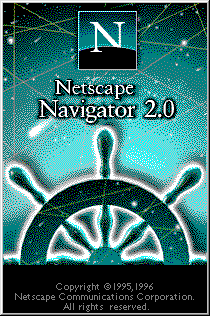
\includegraphics[scale=0.5]{imagenes/netscape.png}
\end{center}
Se produjo una ola de confusión entre programadores al creer que JavaScript era una nueva implementación de Java. Este hecho fue considerado como una estrategia comercial en los momentos de competencia que atravesaba la empresa NetScape al reconocer que Java era uno de los lenguajes más utilizados.\\\\
En 1996, JavaScript fue tomado por la organización ECMA para establecer un estandar y asi otras compañias puedan implementar con el trabajo hecho por NetScape. Se dió origen a ECMAScript el estandar oficial donde JavaScript es uno de sus implementaciones y también se destaca entre ellas ActionScript 3.\\\\
\begin{center}

\includegraphics[scale=0.5]{imagenes/ecma.JPG}
\end{center}
Los procesos de estandarización continuaron dando como resultado ECMAScript 2 y ECMAScript 3 siendo este último la base del actual JavaScript.\\
Se originó la idea de crear una nueva versión de JavaScript llamado el JS2 o conocido como el ES4 original, esta idea fue dirigida por Waldemar Horwat en el 2000, luego tomó el mando NetScape y en la actualidad esta bajo el comando de Google.\\\\
Microsoft también participó e incluso implemento algunos de los propuestos en su lenguaje JScript.net. A través del tiempo se dio a conocer que Microsoft no tenia intención alguna de cooperar o implementar JavaScript en su navegador Internet Explorer, tampoco tenian afinidad de competencia. En el año 2003 el lenguaje JS2/ES4 original fue descartado.\\\\
\begin{center}

\includegraphics[scale=0.5]{imagenes/jscript.JPG}
\end{center}
En el 2005 ocurrieron dos grandes eventos en la historia de JavaScript. Primeramente Brendan Eich (creador de JS) y Mozilla se reincorporaron a ECMA como miembros sin fines de lucro y trabajaron en el estándar E4X, ECMA-357, la cual vino de ex-trabajadores de Microsoft. En conjunto con Macromedia el cual estuvo implementando E4X en ActionScript 3 (siendo este un producto del trabajo en el descartado JS2/ES4 original).\\\\
El trabajo se reinició en ECMAScript 4 con la finalidad de estandarizar lo que había en ActionScript 3 e implementarlo en SpiderMonkey. Para este fin Adobe lanzo el producto AVM2, de nombre código Tamarin como un projecto de código abierto. Tamarin y AS3 eran muy diferentes para su convergencia en la web de JavaScript.\\
Existía conflicto interno entre varios miembros, donde Doug Crockford se unió con Microsoft en el año 2007 para oponerse a ECMAScript 4, produciendose una degradación y originandosé el ECMAScript 3.1.\\\\
Se juntaron varios grupos en Oslo en Julio del año 2008, aquella reunión produjo un acuerdo eventual para renombrar ECMAScript 3.1 a ECMAScript 5 y seguir adelante con el proyecto usando una agenda conocida como Harmony.\\
El resultado de todos estos eventos dieron origen al JavaScript de hoy en día, totalmente innovador y compuesto con nuevas utilidades y herramientas.\\



\section{TUTORIAL DE INSTALACIÓN}
 Desde que los navegadores incluyen el Javascript, no necesitamos el Java Runtime Environment (JRE), para que se ejecute.
\\  \\
Como habilitar JavaScript en tu navegador 
Ahora ya todas las páginas web contienen  JavaScript, un lenguaje de programación que se ejecuta en el navegador web del visitante. \\\\
Con esto se crean páginas específicas en las páginas web y si es desactivada o deja de funcionar por cualquier motivo la página web puede verse limitada o no quedar disponible.
\\\\
Veremos como habilitar(activar) JavaScript en cuatro de los navegadores mas utilizados:
\newline
\newline* Google Chrome
\newline* Mozilla Firefox
\newline* Internet Explorer
\newline
* Opera
\newpage
\begin{figure}
\subsection{Google Chrome}
Aquí veremos como activar JS en uno de los navegadores mas populares y utilizados por los usuarios que es Google Chrome 


\begin{center}
\begin{center}
Navegar google Chrome
\end{center}

\includegraphics[height=3 cm, width=3 cm] {imagenes/chrome.JPG}

\ Imagen 1
\ label { http://www.enable-javascript.com/images/chrome.gif }
\newline
\newline
\begin{center}

\bf PASO 1 
 En el navegador web, haz click en el menú ''Customize and control Google Chrome'' 
y luego selecciona "Settings".
\end{center}

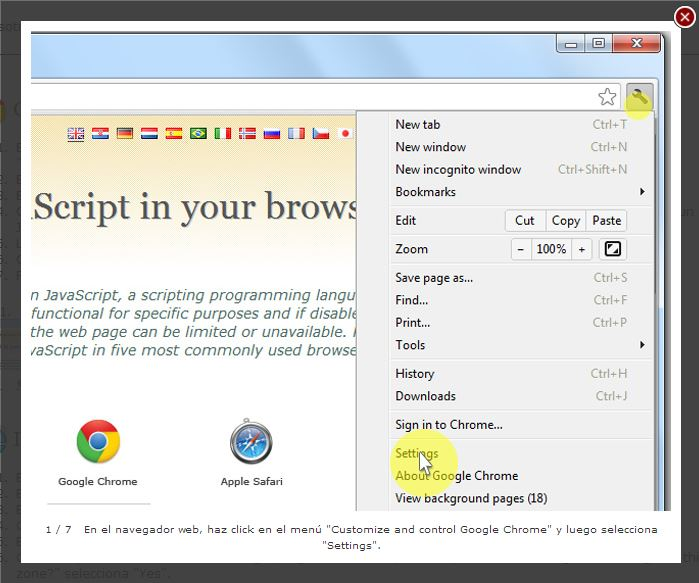
\includegraphics[height=8cm, width=8 cm] {imagenes/chrome 01.JPG}
\newline
\  Imagen 2
\ label { http://www.enable-javascript.com/images/chrome.gif }
\newline

\end{center}
\end{figure}

\begin{figure}
\begin{center}
\begin{center}


\bf PASO 2
En la sección "Settings" haz click en la 
opción "Show advanced settings..."
\end{center}
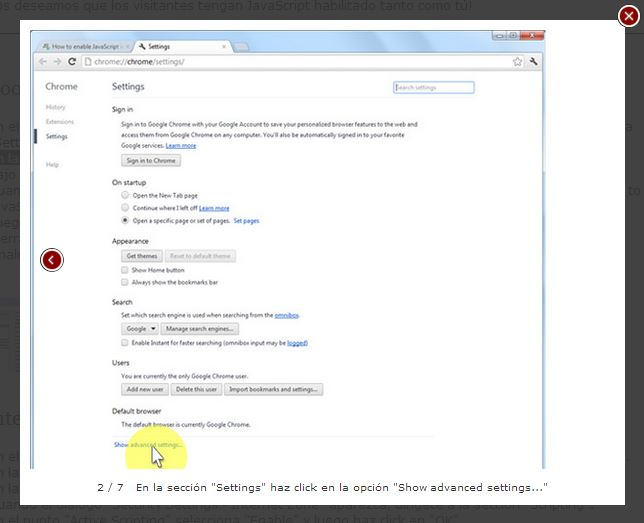
\includegraphics[height=8cm, width=8 cm] {imagenes/chrome 02.JPG}
\newline
\  Imagen 3
\ label { http://www.enable-javascript.com/images/chrome.gif }
\newline




\begin{center}
\bf PASO 3
Bajo la sección "Privacy" haz click en la opción 
``content settings..`` ... (recommended)
\newline
\end{center}
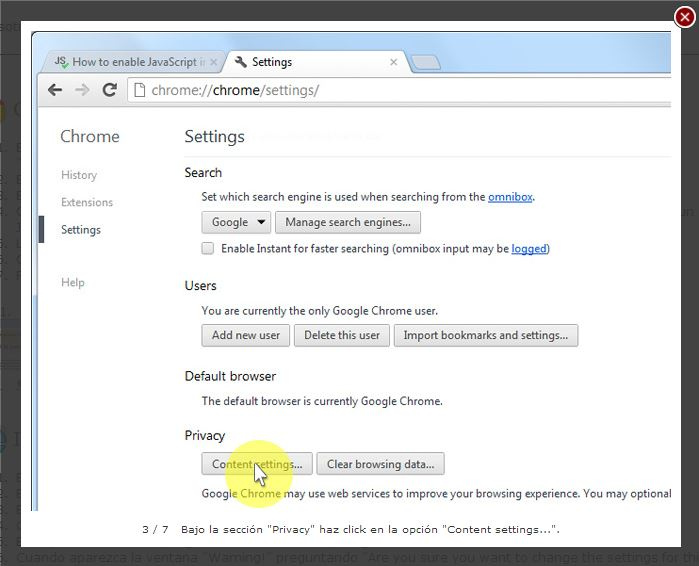
\includegraphics[height=8 cm, width=8 cm] {imagenes/chrome 03.JPG}
\newline
\ Imagen 4
\ label { http://www.enable-javascript.com/images/chrome.gif }
\newline


\end{center}
\end{figure}


\begin{figure}
\begin{center}
\begin{center}

\bf PASO 4
Cuando la ventana aparezca, dirigirse a la sección ``JavaScript``  y seleccionar la opción ``Allow all sites to run JavaScript (recommended)``
\newline
\end{center}

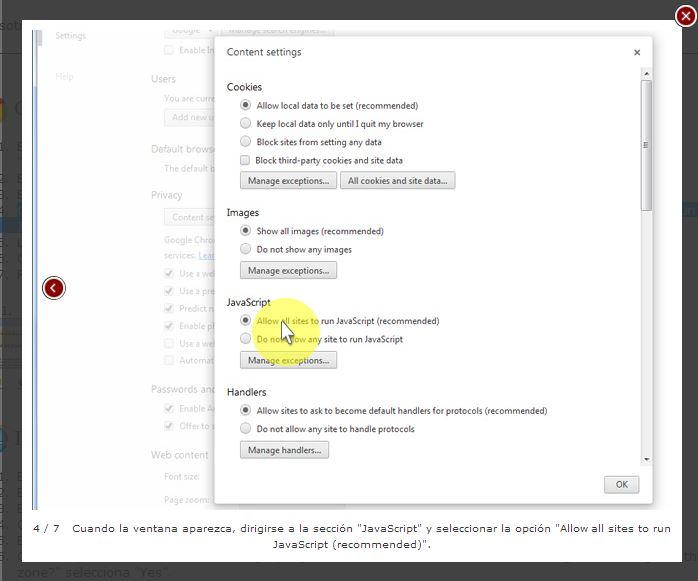
\includegraphics[height=8cm, width=8 cm] {imagenes/chrome 04.JPG}
\newline
\ Imagen 5

\ label { http://www.enable-javascript.com/images/chrome.gif }

\begin{center}
\bf PASO 5
Luego haz click en el botón ``OK`` para cerrar la ventana. (recommended)
\newline
\end{center}

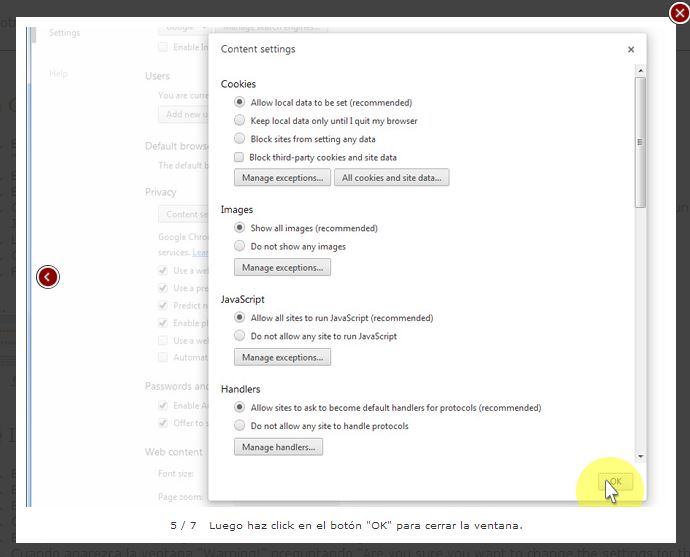
\includegraphics[height=8cm, width=8 cm] {imagenes/chrome 05.JPG}
\newline
\newline
\ Imagen 6
\ label { http://www.enable-javascript.com/images/chrome.gif }
\newline
\end{center}
\end{figure}

\begin{figure}
\begin{center}
\begin{center}

\bf PASO 6 Cierra la pestaña "Settings".
\end{center}

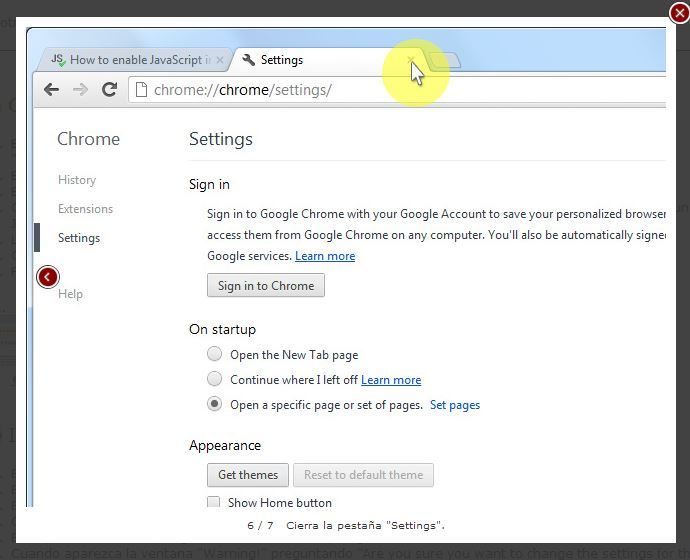
\includegraphics[height=8cm, width=8 cm] {imagenes/chrome 06.JPG}
\newline
\newline
\ Imagen 7
\ label { http://www.enable-javascript.com/images/chrome.gif }


\end{center}
\end{figure}


\begin{figure}
\begin{center}
\begin{center}
\bf PASO 7
Finalmente haz click en el botón ``Reload this page`` del navegador web para refrescar la página.
\newline
\end{center}

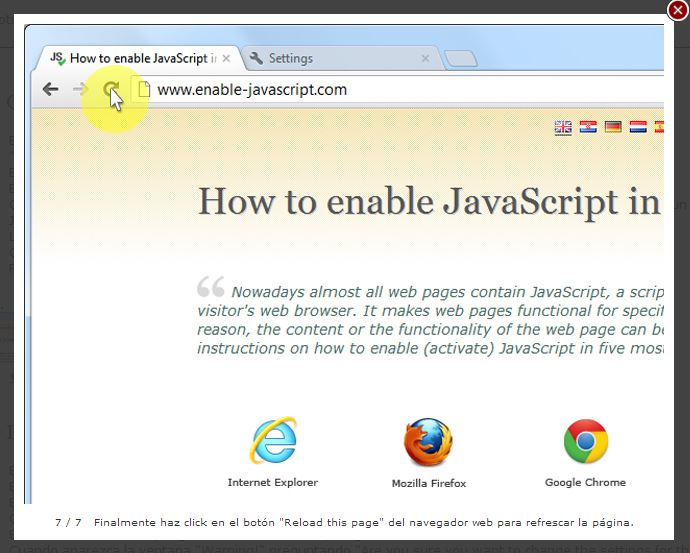
\includegraphics[height=8cm, width=8 cm] {imagenes/chrome 07.JPG}
\newline
\ Imagen 8
\ label { http://www.enable-javascript.com/images/chrome.gif }
\end{center}
\end{figure}


\begin{figure}
\subsection{Mozilla FireFox}

Ahora mostraremos los pasos para otro navegador popular como el Mozilla FireFox
\begin{center}
\begin{center}
Navegar Mozilla Firefox

\end{center}
\begin{center}

\includegraphics[height=3 cm, width=3 cm] {imagenes/firefox.JPG}
\end{center}


\ Imagen 9
\ label {http://www.enable-javascript.com/images/firefox.gif }

\begin{center}
\bf PASO 1 
En el navegador web, has click en el menú ``Firefox`` y luego selecciona el item ``Tools``
y luego selecciona ``Settings``
\end{center}

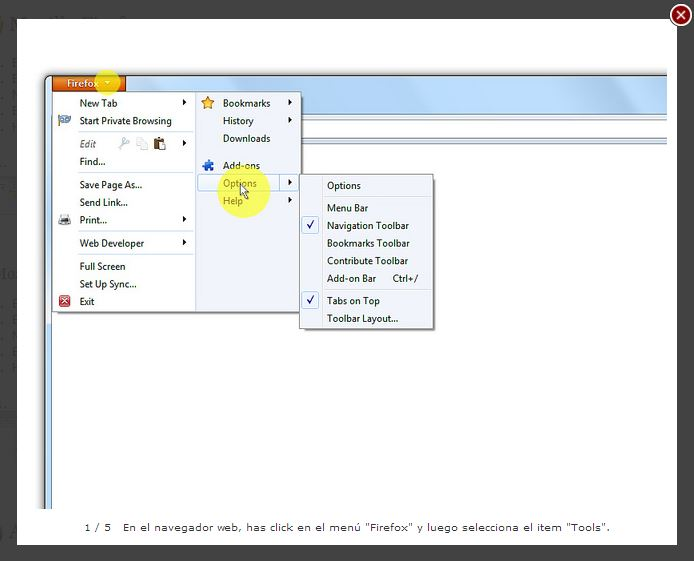
\includegraphics[height=8 cm, width=8 cm] {imagenes/firefox 01.JPG}
\newline
\newline
\ Imagen 10
\ label {http://www.enable-javascript.com/images/firefox.gif }

\begin{center}
\bf PASO 2
En la ventana ``Options`` selecciona la pestaña ``Content``.
\end{center}

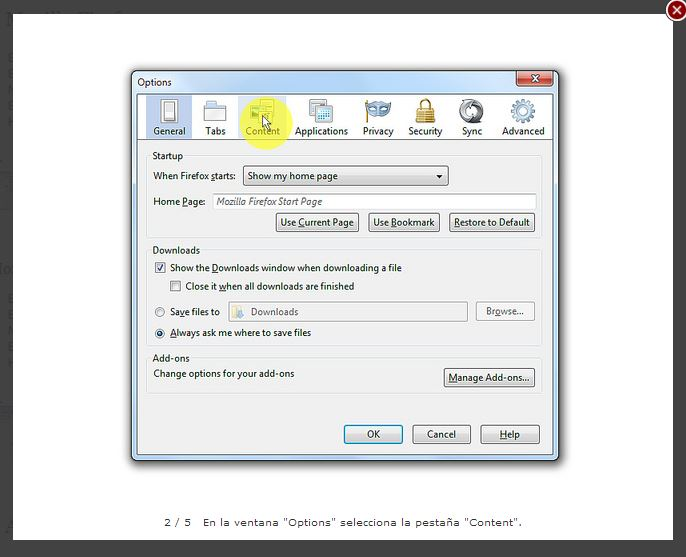
\includegraphics[height=8 cm, width=8 cm] {imagenes/firefox 02.JPG}
\newline
\newline
\ Imagen 11
\ label {http://www.enable-javascript.com/images/firefox.gif }

\end{center}
\end{figure}

\begin{figure}
\begin{center}

\begin{center}
\bf PASO 3
Marca la casilla ``Enable JavaScript``
\newline
\end{center}
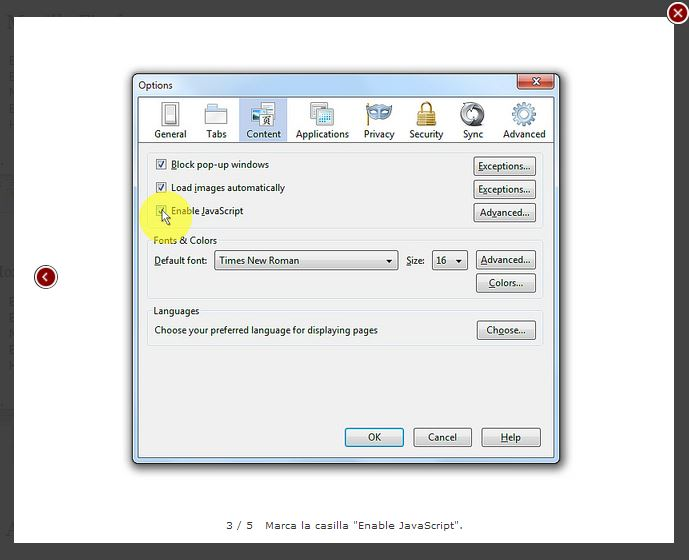
\includegraphics[height=8 cm, width=8 cm] {imagenes/firefox 03.JPG}
\newline
\newline
\ Imagen 12
\ label {http://www.enable-javascript.com/images/firefox.gif }

\begin{center}
\bf PASO 4
En la ventana `` Options`` (ya abierta) haz click en el botón ``OK`` para cerrarla.
\end{center}
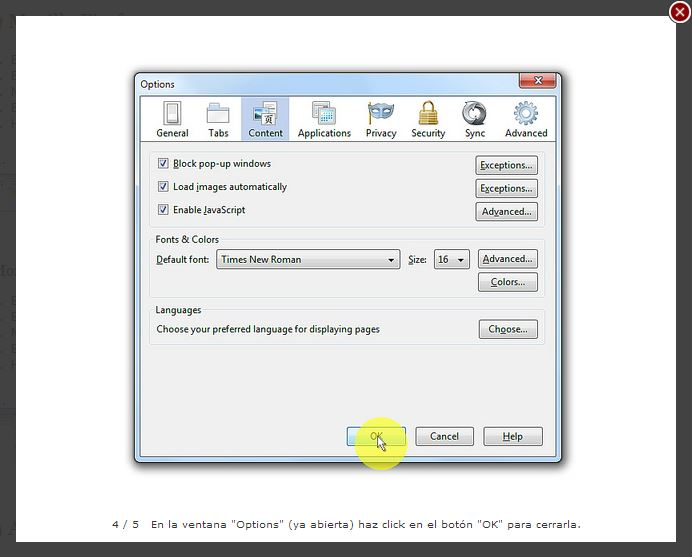
\includegraphics[height=8 cm, width=8 cm] {imagenes/firefox 04.JPG}
\newline
\newline
\ Imagen 13
\ label {http://www.enable-javascript.com/images/firefox.gif }

\end{center}
\end{figure}

\begin{figure}
\begin{center}
\begin{center}
\bf PASO 5
Haz click en el botón ``Reload current page`` del navegador para recargar la página.
\newline
\end{center}
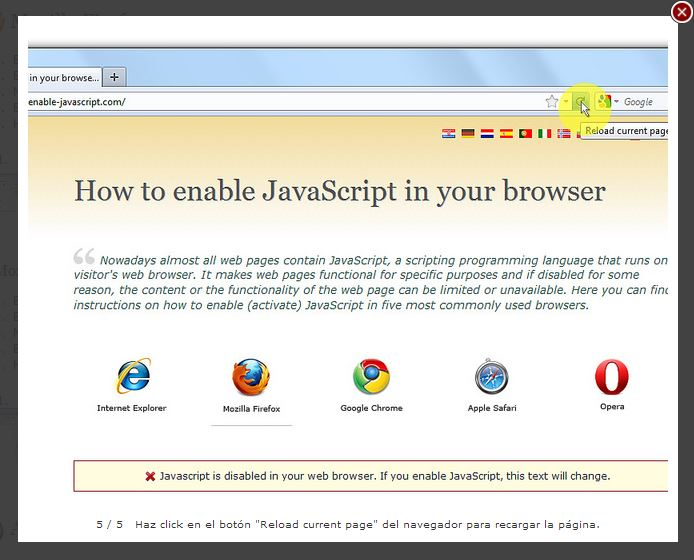
\includegraphics[height=8 cm, width=8 cm] {imagenes/firefox 05.JPG}
\newline
\newline
\ Imagen 14
\ label {http://www.enable-javascript.com/images/firefox.gif }

\end{center}
\end{figure}

\begin{figure}
\subsection{Internet Explorer}
Pasos para activar JavaScript en internet explorer
\begin{center}
\begin{center}
Navegar Internet Explorer

\end{center}
\begin{center}

\includegraphics[height=3 cm, width=3 cm] {imagenes/explorer.JPG}
\end{center}

\ Imagen 15
\ label {http://www.enable-javascript.com/images/ie9.gif }

\end{center}
\end{figure}


\begin{figure}
\begin{center}
\begin{center}
\bf PASO 1
En el menú del navegador web, has click en el icono ``Tools`` y selecciona la opción ``Internet Options``
\end{center}
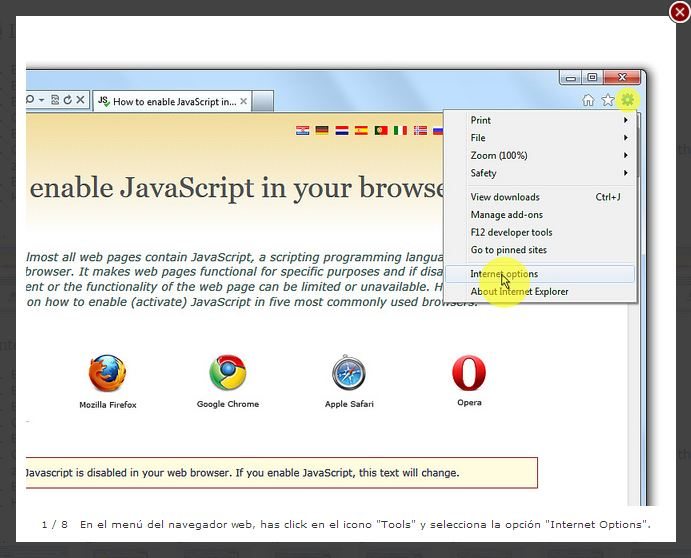
\includegraphics[height=8 cm, width=8 cm] {imagenes/explorer 01.JPG}
\newline
\newline
\ Imagen 16
\ label {http://www.enable-javascript.com/images/ie9.gif }

\begin{center}
\bf PASO 2
En la ventana ``Internet Options`` selecciona la pestaña ``Security``.
\end{center}

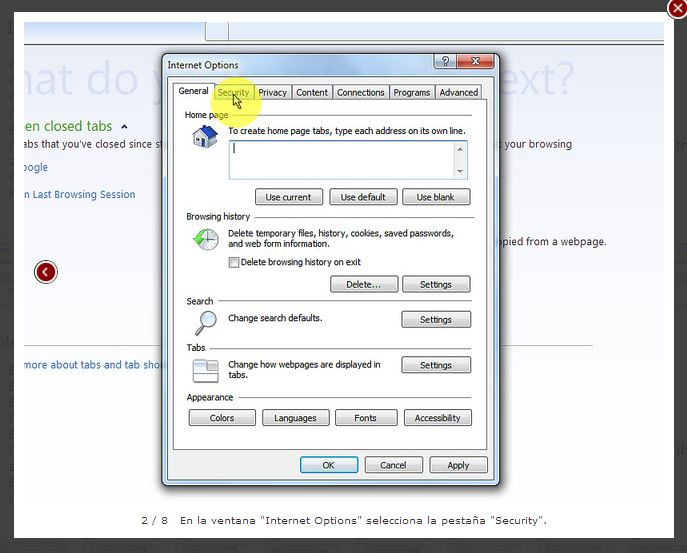
\includegraphics[height=8 cm, width=8 cm] {imagenes/explorer 02.JPG}
\newline
\newline
\ Imagen 17
\ label {http://www.enable-javascript.com/images/ie9.gif }

\end{center}
\end{figure}

\begin{figure}
\begin{center}

\begin{center}
\bf PASO 3
En la pestaña ``Security`` haz click en el botón ``Custom level...``
\end{center}
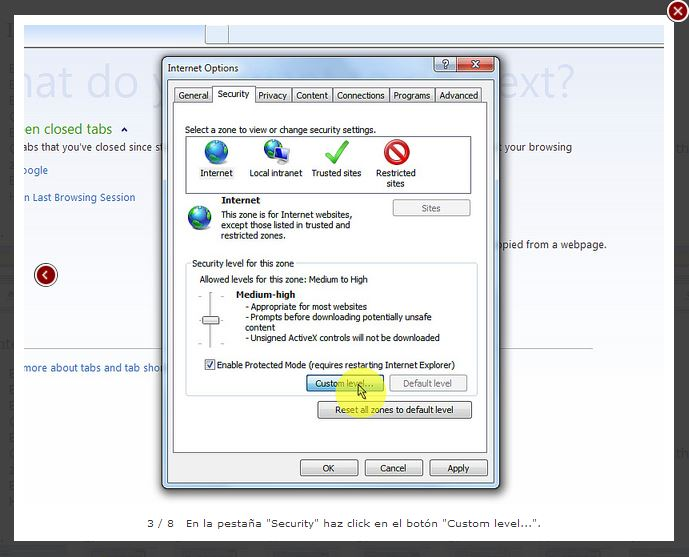
\includegraphics[height=8 cm, width=8 cm] {imagenes/explorer 03.JPG}
\newline
\newline
\ Imagen 18 
\ label {http://www.enable-javascript.com/images/ie9.gif }
\newline
\begin{center}
\bf PASO 4
Cuando el diálogo ``Security Settings - Internet Zone`` aparezca, dirígete a la sección ``Scripting``
\end{center}
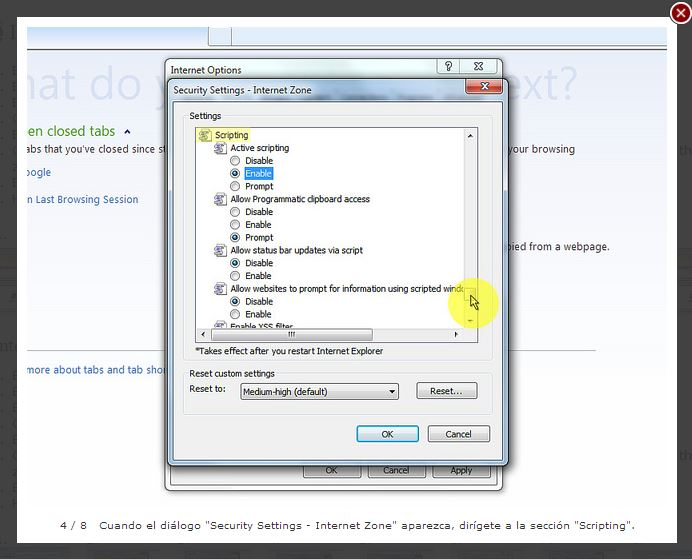
\includegraphics[height=8 cm, width=8 cm] {imagenes/explorer 04.JPG}
\newline
\newline
\ Imagen 19
\ label {http://www.enable-javascript.com/images/ie9.gif }

\end{center}
\end{figure}


\begin{figure}
\begin{center}

\begin{center}
\bf PASO 5
En el punto ``Active Scripting`` selecciona ``Enable`` y luego haz click en ``OK``
\end{center}
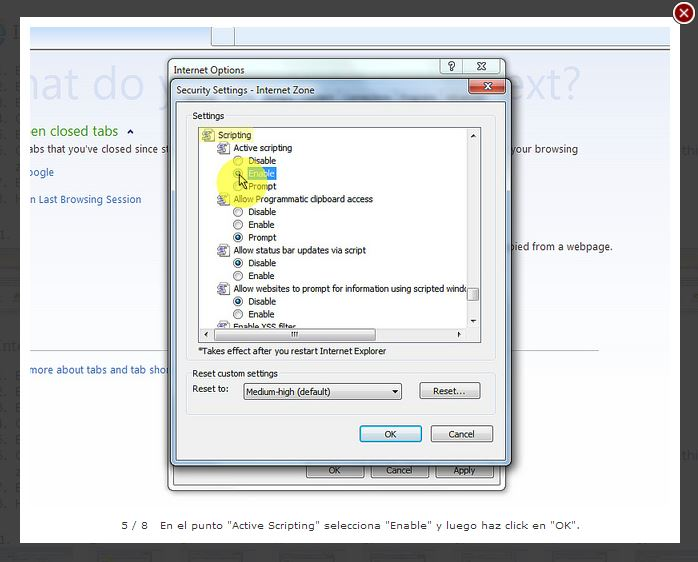
\includegraphics[height=8 cm, width=8 cm] {imagenes/explorer 05.JPG}
\newline
\newline
\ Imagen 20
\ label {http://www.enable-javascript.com/images/ie9.gif }
\newline

\begin{center}
\bf PASO 6
Cuando aparezca la ventana ``Warning!``  preguntando  ``Are you sure you want to change the settings for this zone?  selecciona ``Yes``
\end{center}
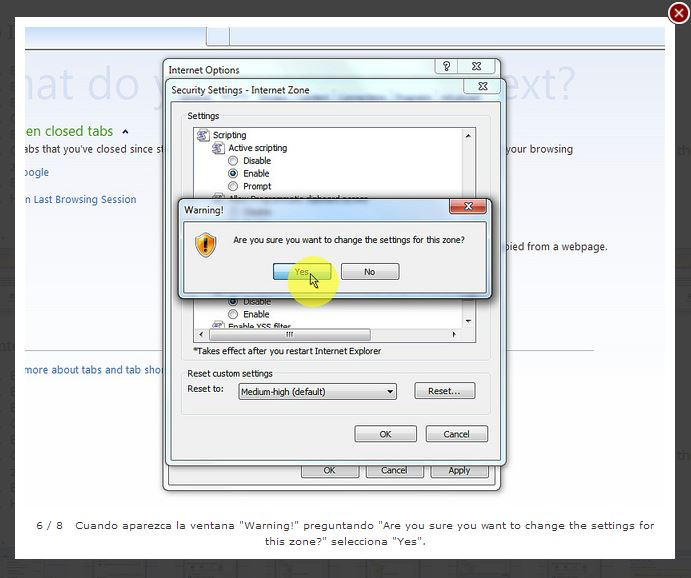
\includegraphics[height=8 cm, width=8 cm] {imagenes/explorer 06.JPG}
\newline
\newline
\ Imagen 21
\ label {http://www.enable-javascript.com/images/ie9.gif }

\end{center}
\end{figure}


\begin{figure}
\begin{center}

\begin{center}
\bf PASO 7
En la ventana ``Internet Options`` haz click en el botón ``OK``para cerrarla.
\end{center}
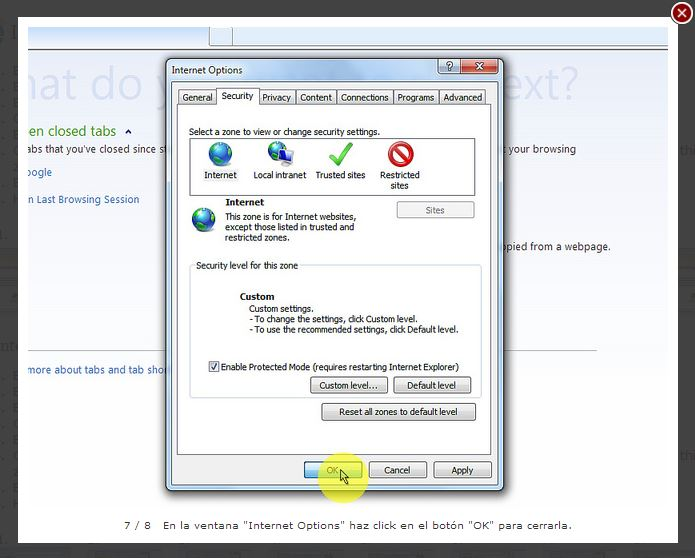
\includegraphics[height=8 cm, width=8 cm] {imagenes/explorer 07.JPG}
\newline
\newline
\ Imagen 22
\ label {http://www.enable-javascript.com/images/ie9.gif }

\begin{center}
\bf PASO 8
Haz click en el botón ``Refresh`` del navegador para recargar la página.
\end{center}

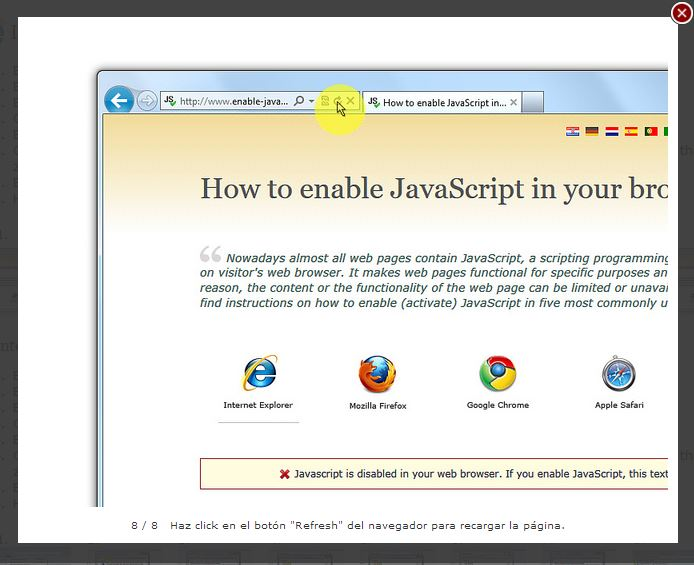
\includegraphics[height=8 cm, width=8 cm] {imagenes/explorer 08.JPG}
\newline
\newline
\ Imagen 23
\ label {http://www.enable-javascript.com/images/ie9.gif }

\end{center}
\end{figure}


\begin{figure}
\subsection{Navegador Opera}
Pasos para activar JavaScript en navegador Opera
\begin{center}
\begin{center}
Navegar Opera

\end{center}
\begin{center}
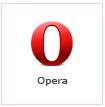
\includegraphics[height=3 cm, width=3 cm] {imagenes/opera.JPG}
\end{center}

\ Imagen 24
\ label {http://www.enable-javascript.com/images/opera.gif}
\newline

\begin{center}
\bf PASO 1
a) Haz click en el botón ``Menu`` del navegador web. En las opciones que aparecen, dirígite a ``Settings``, luego a ``Quick preferences`` y marca la casilla ``Enable JavaScript``.
\end{center}
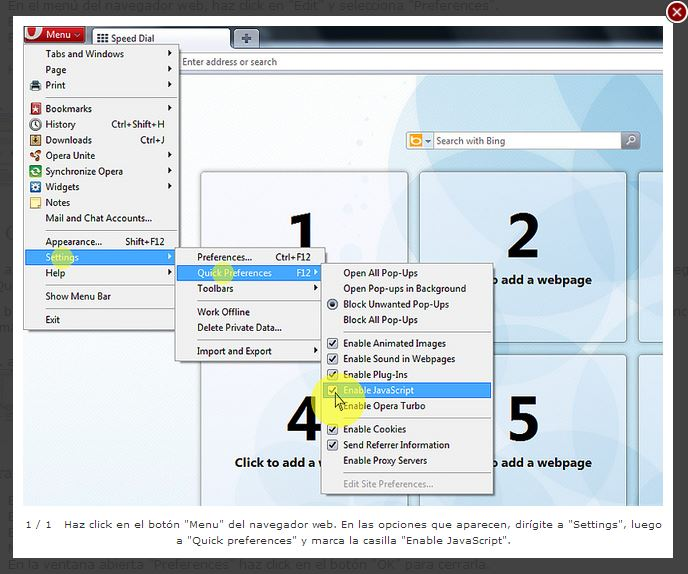
\includegraphics[height=8 cm, width=8 cm] {imagenes/opera 01.JPG}
\newline
\newline
\ Imagen 25
\ label {http://www.enable-javascript.com/images/opera.gif}

\end{center}
\end{figure}

\begin{figure}
\begin{center}

\begin{center}
\bf PASO 1
 b) Si el "Menu bar" se encuentra, haz click en la opción ``Tools`` del navegador web, luego a ``Quick preferences`` y marca la casilla ``Enable JavaScript``.
\end{center}

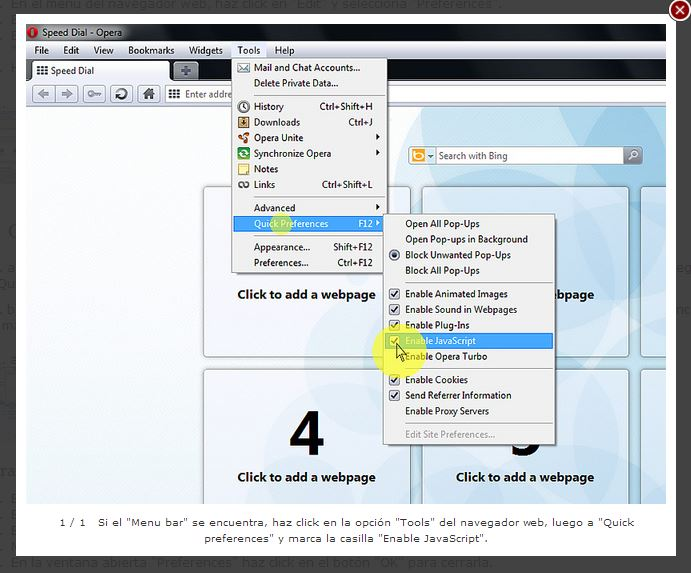
\includegraphics[height=8 cm, width=8 cm] {imagenes/opera 02.JPG}
\newline
\newline
\ Imagen 26
\ label {http://www.enable-javascript.com/images/opera.gif}



\section{Hola Mundo y otros Programas Introductorios} 

Con javascript podemos hacer páginas dinámicas dando versatilidad al usuario que navega en un sitio web. Podemos realizar páginas transaccionales y crear eventos con gran facilidad.


\fbox{ 
function funcionEjemplo() 
\{
alert("Hello World!  :D ");
\}
 }

En este lenguaje podemos usar muchas o casi todas las funciones y caracteristicas de Java ya que es un discipulo del mismo, por lo tanto este lenguaje nos permite realizar constructores con la misma sintaxis de java común.

\fbox{ 
function Persona(firstname,lastname,age,eyecolor)
\{
this.firstname=firstname;
this.lastname=lastname;
this.age=age;
this.eyecolor=eyecolor;
\}
 }

Se hace uso del DOM en algunos codigos de Javascript
\fbox{ 
document.getElementById("demo").innerHTML="Hello Dolly";
document.getElementById("myDIV").innerHTML="How are you?";
}

\end{center}


\section{Bibliografía}


\  {http://www.w3schools.com/js }

\  {http://aprendeenlinea.udea.edu.co/lms/ova/mod/resource/view.php?id=1598 }

\  {http://lenguajesscript.blogspot.com/2012/09/caracteristicas-principales-del.html }

\ {Historia: http://en.wikipedia.org/wiki/JavaScript} 

\ {Historia: http://www.w3.org/community/webed/wiki}
\end{figure}


\lstset{language=Pascal}          % Set your language (you can change the language for each code-block optionally)




\end{document}